%%
% Please see https://bitbucket.org/rivanvx/beamer/wiki/Home for obtaining beamer.
%%
\documentclass{beamer}
\usepackage[backend=bibtex,sorting=none]{biblatex}
\addbibresource{mybeamer.bib} 
\usepackage{multirow}
\usepackage[ruled,linesnumbered]{algorithm2e}
\usepackage{algorithmic}
\usepackage{subfigure}
\usepackage{float}
%\setbeamerfont{footnote}{size=\small}
\begin{document}
\title[Adam-CBO]{A CONSENSUS-BASED GLOBAL OPTIMIZATION
METHOD WITH ADAPTIVE MOMENTUM ESTIMATION}
\frame{\titlepage}

\begin{frame}<beamer>
	\frametitle{\textbf{Outline}}
	\tableofcontents[]
\end{frame}

\section{Why Zero Order Method}
\begin{frame}
	\frametitle{Why Zero Order Method}
	First Order Method (gradient based) is widely used in Machine learning problems, including 
	SGD, SGD momentum, AdaGrad, and  Adam and so forth.
	The problems of Gradient based method 
	\begin{itemize}
		\item Most gradient-based methods have problems dealing with functions that have large noise or non-differentiable functions.
		\item  It has been proved that as the
		deep neural network gets deeper, the gradient tends to explode or vanish.\footfullcite{hanin2018neural}
		\item It will be easily influenced by the geometry of the landscape\footfullcite{liu2020bad}
	\end{itemize}
\end{frame}

\begin{frame}
	\frametitle{Gradient-free methods}
	There are also gradient-free methods such as
	\begin{itemize}
		\item Nelder-Mead (NM)
		\item genetic algorithm (GA)
		\item simulated annealing (SA)
		\item particle swarm optimization (PSO)
	\end{itemize}
\end{frame}

\section{CBO Method}
\begin{frame}
	\frametitle{The original CBO method}
   CBO\footfullcite{carrillo2018analytical}\footfullcite{totzeck2018numerical}\footfullcite{pinnau2017consensus} is based on interacting particle system, along the line of consensus based models. 
   During the dynamic evolution, the particle system tends to their weighted average, and meanwhile undergoes some fluctuation due to the random noise, such as the isotropic geometric Brownian motion
   
\end{frame}

\begin{frame}
	   Consider N particles, labeled as $X^i$, $i =1 , \cdots N$,
   \begin{equation}
   	\begin{aligned}
   		\dot X^i = -\lambda (X^i - \bar{x}^*) +\sigma |X^i-\bar{x}^*| \dot W^i
   	\end{aligned}
   \end{equation}
   $\bar{x}^* = \frac{1}{\sum_{i=1}^N e^{-\beta L(X^i)}}\sum_{i=1}^N X^i e^{-\beta L(X^i)}$ : weighted average of the position of the particle\\
   $L$: cost function \\
   $\dot W$: white noise.\\
  Discretize the above system as follows 
     \begin{equation}
   	\begin{aligned}
   		X^i_{t+1} =  X^i_{t} -\lambda (X^i - \bar{x}^*) +\sigma |X^i-\bar{x}^*|  W^i
   	\end{aligned}
   \end{equation}
\end{frame}

\begin{frame}
\frametitle{Curse of Dimension of original CBO method}
	The convergence was proved in with exponential rate in time under dimension-dependent conditions, i.e., the learning rate depends on the dimension. \\
	Therefore, the CBO method may suffer from the curse of dimensionality.\\
To overcome this issue, \footfullcite{carrillo2019consensus} proposed to replace the isotropic geometric Brownian motion with the component-wise one.

 Such a modification leads to the convergence to the global minimizer with dimension-independent parameters. 
\end{frame}
\begin{frame}
	\frametitle{Problem of CBO}
	\begin{itemize}
		\item Dependent on the initial data
		\item Hard to optimize high dimensional no-convex function, like Rastrigin Function over $20$ dimension.
		\item Hard to optimize deep neural network, for too much parameters.
	\end{itemize}
\end{frame}
\section{Adam CBO Method}
\begin{frame}
	\frametitle{First Order Momentum}
	We consider model
	\begin{equation}
    \sigma \ddot X^i_t + \dot X^i_t = -(X_t- x^*) , \quad i=1,\cdots,N, \label{eqn:2ndsystem}
\end{equation}
It can be written into a first order PDE system
\begin{align*}
    &\dot X_t^i = -M_t^i, \\
    &\sigma \dot M_t^i + M_t^i = X_t^i - x^*.
\end{align*}
can be further simplified as
\begin{align}
&X^i_{t+1} = X_t^i -\delta t M^i_{t+\frac{1}{2}},\\
&M^i_{t+\frac{1}{2}} = \frac{\sigma - \delta t}{\sigma+ \delta t}M_{t-\frac{1}{2}} + \frac{2\delta t}{\sigma  + \delta t } (X_t^i - x^*).
\end{align}
\end{frame}
\begin{frame}
It's trivial that we can find parameters that satisfy the $\lambda = \delta t $ and $\beta_1 =\frac{\sigma - \delta t}{\sigma+ \delta t} =1 - \frac{2\delta t }{\sigma  + \delta t }  $.
	\begin{equation}
		\begin{aligned}
&X^i_{t+1} = X_t^i - \lambda M^i_{t+1}  \\
\ &M^i_{t+1} = \beta_1 M^i_{t} + (1-\beta_1) (X_t^i - \bar{x}^*).
		\end{aligned}
	\end{equation}
	Since $\delta t$ is a small number, we have $\beta_1$ is near 1 ($=0.9$ in practice).
	Similar with the CBO method, we add the stochastic terms in the model,
	\begin{equation}
		\begin{aligned}
&X^i_{t+1} = X_t^i - \lambda M^i_{t+1} + \sigma_t  W^i_t \\
\ &M^i_{t+1} = \beta_1 M^i_{t} + (1-\beta_1) (X_t^i - \bar{x}^*)+\gamma_t  \xi^i_t.
	\end{aligned}
	\end{equation}
Notice that the $\xi_t$ don't need to add artifically, since the calculation of $\bar{x}^*$ in optimization with random sampling, already introduce stochastic term in momentum equation.
	\end{frame}
	\begin{frame}
	\frametitle{The connection between CBO momentum method and original one}
	In Exception means,
	\begin{equation}
		\begin{aligned}
			X^i_{t+1} &= X_t^i - \lambda M^i_{t+1} + \sigma_t W^i_t \\
			&\downarrow\\
			\dot X^i_{t+1} &= X_t^i  -\lambda (X^i - \bar{x}^*) +\sigma |X^i-\bar{x}^*|  W^i
		\end{aligned}
	\end{equation}
	
	
The $M_t^i$ can is the moving average $X_{t}^i - x^*$
\begin{equation*}
	\begin{aligned}
		M^i_t & = \beta_1 M^i_{t-1} + (1-\beta_1)(X^i_{t-1} - x^*)\\
		& = \beta_1 (\beta_1 M^i_{t-2} + (1-\beta_1) (X_{t-1}^i - x^*)) + (1-\beta_1) (X^i_{t-2} - x^*)\\
		& = \cdots \\
		& = (1-\beta_1) \sum_{k=0}^{t-1} \beta_1^{t-k} (X_{k}^i - x^*).
	\end{aligned}
\end{equation*}
\end{frame}
\begin{frame}
	\begin{equation*}
	\begin{aligned}
		\mathbb{E} [M^i_t] & =(1-\beta_1)   \mathbb{E} [\sum_{k=0}^t \beta_1^{t-k} (X_{k}^i - x^*)] \\
		&= (1-\beta_1) \mathbb{E}[ X_{t}^i - x^* ]  \sum_{k=0}^t \beta_1^{t-k} \\
		&= (1-\beta_1^t)  \mathbb{E}[ X_{t}^i - x^* ].
	\end{aligned}
\end{equation*}
To get an unbiased estimation of $ (X_{k}^i - x^*)$ for small $t$ as well, we rescale $M^i_t$ by $(1-\beta_1^t)$ and denote by $\hat{M}^i_t$. This shows the our method and original one is the same in Exceptation means.
\end{frame}

\begin{frame}
	\frametitle{Second Order Momentum}
	For the second order moment $\mathbb{E}(|X^i_t-x^*|^2)$\footnote{The square here is defined in the element-wise sense.}, we define 
\begin{equation}
	\begin{aligned}
	\label{equ:CBO second order moment}	V^i_t  = \beta_2 V^i_{t-1} + (1-\beta_2) |X^i_t - x^*|^2. 
	\end{aligned}
\end{equation}
Application of the same argument for $\mathbb{E}[X^i_t]$ yields
\begin{equation}
	\mathbb{E}[V^i_t] = (1-\beta_2^t) \mathbb{E}[|X^i_t-x^*|^2],
\end{equation}
and $\hat{V}^i_t = \frac{V^i_t}{1-\beta_2^t}$ is an unbiased estimation of $\mathbb{E}[|X^i_t- x^*|^2]$. Therefore, we modify the model into 
\begin{equation}
	\begin{aligned}
	\label{equ: CBO moment model true}	X^i_{t+1} = X_t^i - \frac{\lambda \hat{M}^i_{t+1}}{\sqrt{\hat{V}^i_{t+1}} + \epsilon} + \sigma^ t  W_t^i,
	\end{aligned}
\end{equation}
where $\epsilon$ is a small number and typically takes the value $1e-8$ to avoid the vanishing of the denominator.
\end{frame}
\begin{frame}
\small{
\begin{algorithm}[H]
\KwIn{$\lambda$, $N$, $M$, $t_N$, $\beta_1$, $\beta_2$}

  Initialize $X^i_0$, $i = 1,\cdots N$ by the uniform distribution;
  
  Initial $M^i_0,V^i_0 =0$;
  \tcc{Initialize first order and second order moments.}
  
  \For{$t = 0$ \textbf{to} $t_N$ }{
    Generate a random permutation of index $\{1,2,\cdots,N\}$ to form set  $P_k$;
    
    Generate batch set of particles in order of $P_k$ as $B^1,\cdots B^{\frac{N}{M}}$ with each batch having $M$ particles;
    
    \For{$j = 0$  \textbf{to} $\frac{N}{M}$}{
        Update $x^* =\sum\limits_{k\in B^j} \frac{X_t^k\mu^k_t}{\sum\limits_{i\in B^j} \mu_t^i }$, where $\mu_t^i = \omega_f^\alpha (X_t^i)$;
        
        Update $X^i_t$ for $j \in B^j$ as follows
        
        $
        M^i_{t+1} = \beta_1 M_{t}^i +(1-\beta_1) (X^i_t-x^*) \quad \quad \hat{M}^i_{t+1} = M^i_{t+1}/(1-\beta_1^t)
        $;
        
        $
        V^i_{t+1} = \beta_2 V_{t}^i +(1-\beta_2) (X^i_t-x^*)^2 \quad \quad  \hat{V}^i_{t+1} = V^i_{t+1}/(1-\beta_2^t)
        $;
        
        $
        X^i_{t+1} = X^i_t - \lambda \hat{M^i_t}/(\sqrt{\hat{V^i_t}}+\epsilon) + \sigma^t \sum_{k = 1}^d \vec{e}_k z_i  \quad z_i\; \text{ is a random variable}
        $.
    }
    }
    \KwOut{$X_{t_N}^i, \quad i = 1\cdots N$}
  \label{alg:CBO-moment}
\end{algorithm}
}
\end{frame}
\begin{frame}
	\frametitle{A linear stability analysis of the Adam-CBO method}
	 We first rewrite Algorithm into a continuous form and ignore the stochastic term
	\begin{align}
&\dot m = (\beta_1 -1) m + (1-\beta_1) (x-\bar{x}),\\
&\dot v = (\beta_2 -1) v + (1-\beta_2) (x-\bar{x})^2,\\
&\hat{m} = \frac{m}{1-\beta_1^t} \quad  \hat{v} = \frac{v}{1-\beta_2^t}, \\
&\dot x =  - \lambda \frac{\hat{m}}{\sqrt{\hat{v}}+\epsilon},
	\end{align}

\end{frame}
\begin{frame}
	Denote $\tilde{x} = x - \bar{x}$. Linearizing the system around $m = 0, x = \bar{x}, v = 0 $, we have
	\begin{align}	
	&\dot m = -(1-\beta_1) m + (1-\beta_1) \tilde{x},\\
	&\dot v = -(1-\beta_2)v, \\
	&\dot {\tilde{x}} = -\frac{\lambda }{(1-\beta_1^t)\epsilon}m \rightarrow -\frac{\lambda}{\epsilon} m = -\mu m  \quad (t \rightarrow \infty)
	\end{align}
	with $\mu=\lambda/\epsilon$, and in a vector form,
	\begin{equation}
	\begin{aligned}
	\partial_t	\left(\begin{matrix}
			m \\ v \\ \tilde x
		\end{matrix}\right) = 
	\left(\begin{matrix}
		-(1-\beta_1) & 0 & 1-\beta_1\\ 
		0 &  -(1-\beta_2) & 0  \\
		 -\mu & 0 & 0  
	\end{matrix}\right) 
	\left(\begin{matrix}
	m \\ v \\ \tilde x
	\end{matrix}\right). 
	\end{aligned}
	\end{equation}
\end{frame}

\begin{frame}
\begin{theorem}
	\textbf{Algorithm} generates a sequence that converges to the optimal solution with rates independent of the learning rate $\lambda$. 
	\begin{proof}
	Eigenvalues of the matrix on the right-hand side are $\beta_2-1$ and $\frac{1}{2}( \beta_1 - 1 \pm i  \sqrt{1-\beta_1}\sqrt{\beta_1-1+4\mu})$ (typically $1-\beta_1\ll 4\mu$), respectively. Thus, $m,v,\tilde{x}$ decay to $0$  exponentially with rate $\beta_2 -1 $ when $\beta_1>2\beta_2+1$ and with rate $\frac{1}{2}(\beta_1-1)$ when $\beta_1 < 2 \beta_2 + 1$ in an oscillatory way. 
	\end{proof}
\end{theorem} 	
\end{frame}
\begin{frame}
The CBO method without random noise can be written into a continuous form
\begin{equation}
\dot x = - \lambda (x- \bar{x}).
\end{equation}
The ODE can be solved analytically with a decay rate $e^{-\lambda t }$ towards the stationary point.
Therefore, the decay rate of the CBO method depends exponentially on the learning rate $\lambda$.
\end{frame}

\section{Numerical Example}
\subsection{Rastirgin Function}
\begin{frame}
	\frametitle{Rastrigin Function}
	Finding the global minimizer of the Rastrigin function
\begin{equation}\label{eqn:rastrigin}
	f(x) = \frac{1}{d} \sum_{i=1}^d \left[(x_i-B)^2 -10\cos(2\pi (x_i-B)) + 10\right] + C
\end{equation}
with $B = \arg \min f(x)$ and $C= \min f(x)$. Figure is a visualization of \eqref{eqn:rastrigin} when $d=2$ and $B=C=0$. 

\begin{figure}[ht]
	\centering
	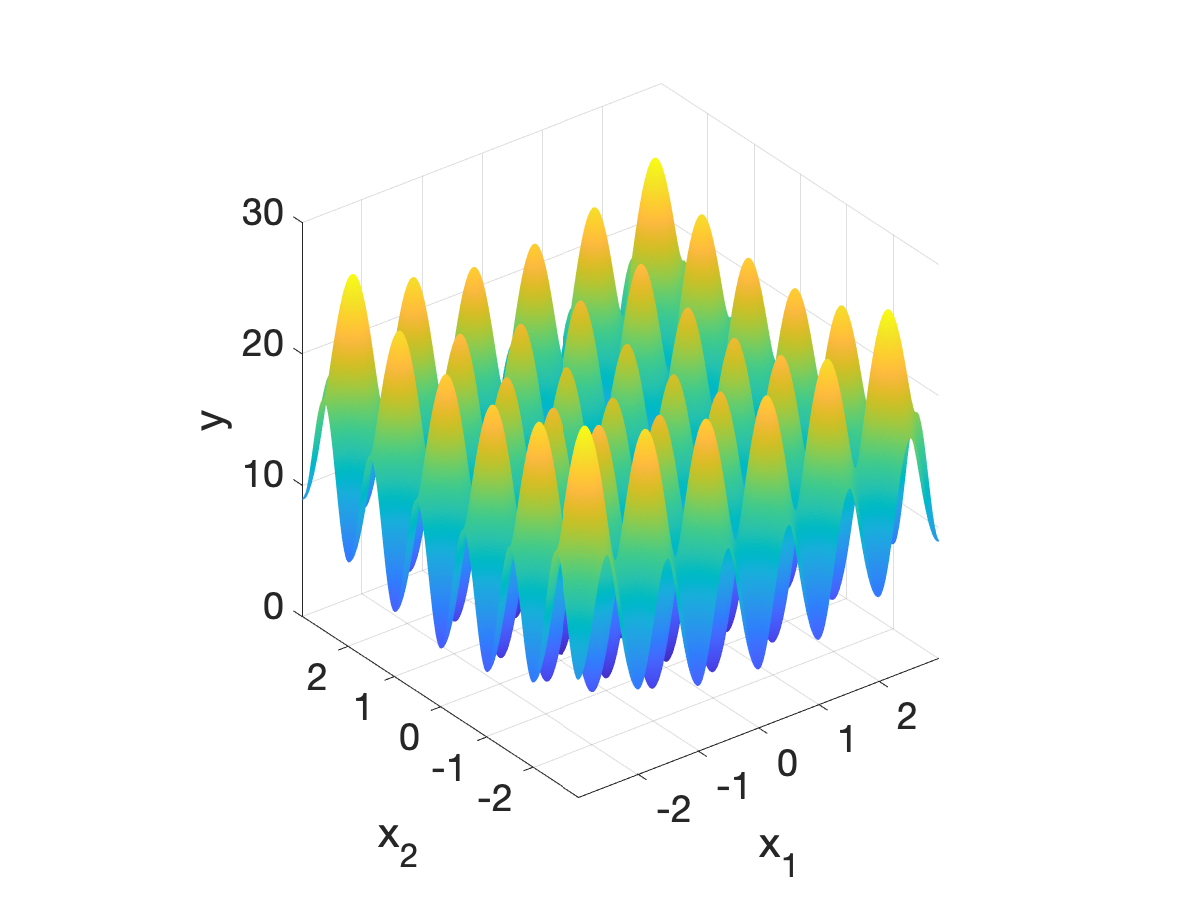
\includegraphics[width=0.6\linewidth]{Figure/R_function}
\end{figure}
\end{frame}

\begin{frame}
	The number of local minima is $5^d$, which grows exponentially fast in term of the dimensionality. When $d=1000$, the number of minima is $5^{1000}$, approximately $10^{690}$.
\begin{table}[ht]

	\centering\begin{tabular}{|c|c|c|c|c|c|}
	\hline
	d & 1 & 2 & 30 & 100 & 1000 \\
	\hline
	Number of local minima & $5$ & $5^2$ & $5^{30}$ & $5^{100}$ & $5^{1000}$\\
	\hline 
	\end{tabular}
	\caption{Number of local minima for the Rastrigin function in terms of dimension.}
	\label{tbl:Number of local minimum}
\end{table}

\end{frame}

\begin{frame}
\begin{table}
	\centering
	\begin{tabular}{|c|c|c|c|c|c|}
		\hline
		\multirow{2}*{$d$}&
		\multirow{2}*{$N$}&
		\multirow{2}*{$M$}&\multicolumn{3}{c|}{CBO}\\
		\cline{4-6}
		~& ~ & ~ &  $\mathcal{N}(0,1)$&$\mathcal{U}(-1,1)$ &Wiener process  \\
		\hline 
		2  & 50 & 40 & 100\% & 100\% & 99\% \\
		10 & 50 & 40 & 100\% & 100\% & 2\%  \\
		20 & 50 & 40 & 98\%  & 22\%  & 0\%  \\
		20 & 50 & 20 & 66\%  & 2\%   & 0\%  \\
		30 & 50 & 40 & 26\%  & 0\%   & 0\%  \\
		30 & 500&5   &  0\%  & 0\%   & 0\%  \\
		%30 & 500 & 400 &     & 0\%   &  \%  \\
		\hline
		\multirow{2}*{$d$}&
		\multirow{2}*{$N$}&
		\multirow{2}*{$M$}&\multicolumn{3}{c|}{Adam-CBO}\\
		\cline{4-6}
		~& ~ & ~ &  $\mathcal{N}(0,1)$& $\mathcal{U}(-1,1)$ &Wiener process  \\
		\hline
		30 & 500  & 5  & 99\% & 100\% & 0\% \\
		100& 5000 & 5  & 100\% & 100\% & 0\%\\
		1000& 8000 & 50 & 92\% & 20\% &0\%\\
		\hline
	\end{tabular}
	\caption{Comparison of CBO and Adam-CBO methods with different random processes.}
	\label{tbl:process sr}
\end{table}	
\end{frame}
\begin{frame}
	\begin{table}
	\centering
	\begin{tabular}{|c|c|c|c|c|}
		\hline
		\multirow{2}*{$d$}&
		\multirow{2}*{$N$}&
		\multirow{2}*{$M$}&\multicolumn{2}{c|}{Adam-CBO}\\
		\cline{4-5}
		~& ~ & ~ &  $\mathcal{N}(0,1)$& $\mathcal{U}(-1,1)$\\
		\hline
		30& 500 &  5  & 94\% & 100\% \\
		100& 5000 & 5  & 100\% & 94\% \\
		1000& 10000 & 50  & 100\% & 11\% \\
		\hline
	\end{tabular}
	\caption{Comparison of success rates for different dimensions when $X^i_t$ is initialized by $0$ ($X^i_0 = 0$), $\lambda = 0.1$, and $\sigma^t= 0.99^{\frac{t}{20}}$.}
	\label{tbl:initial sr}
\end{table}
\end{frame}
\subsection{DNN Approximate function}
\begin{frame}
\frametitle{Frequency Principle}
	Consider two functions
\begin{align}
	\label{equ:target 1} &u(x) = \sin(2\pi x) + \sin(8 \pi x ^2), \\
	\label{equ:target 2} &u(x) = \left\{\begin{matrix}
		1   & x < -\frac{7}{8}, x> \frac{7}{8}, -\frac{1}{8}<x<\frac{1}{8}\\
		-1  & \frac{3}{8}< x< \frac{5}{8} , -\frac{5}{8}< x<- \frac{3}{8}\\
		0 & \text{otherwise} 
	\end{matrix} \right.,
\end{align}
\end{frame}
\begin{frame}
\begin{figure}[ht]
	\centering
	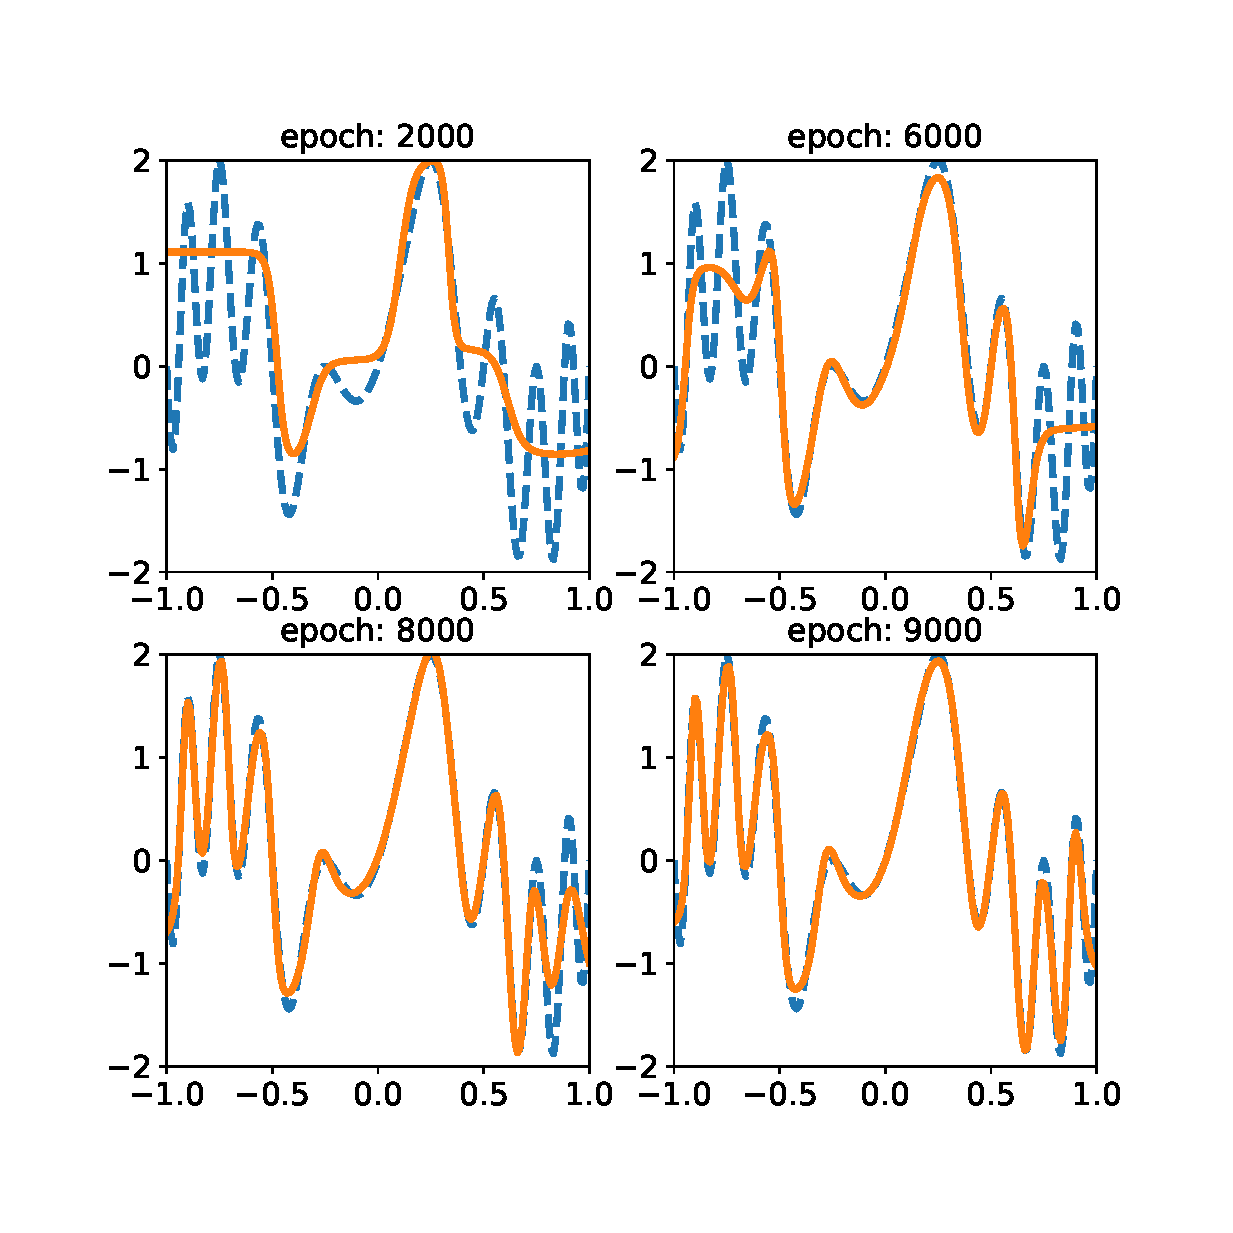
\includegraphics[width=0.6\linewidth]{Figure/Fprinciple_exm1}
	\caption{Approximating function \eqref{equ:target 1} using a network with  width $ = 50$, depth $ = 3$, and $2701$ parameters in total. The learning rate is $\lambda=0.2$. $N = 500$ particles and $M=5$ particles for each batch are used in the first $50000$ iterations. After that, the random term is ignored and $M = 10$ is used for faster convergence to the optimal solution.}
	\label{fig:fprincipleexm1}
\end{figure}	
\end{frame}
\begin{frame}
\begin{figure}[ht]
	\centering
	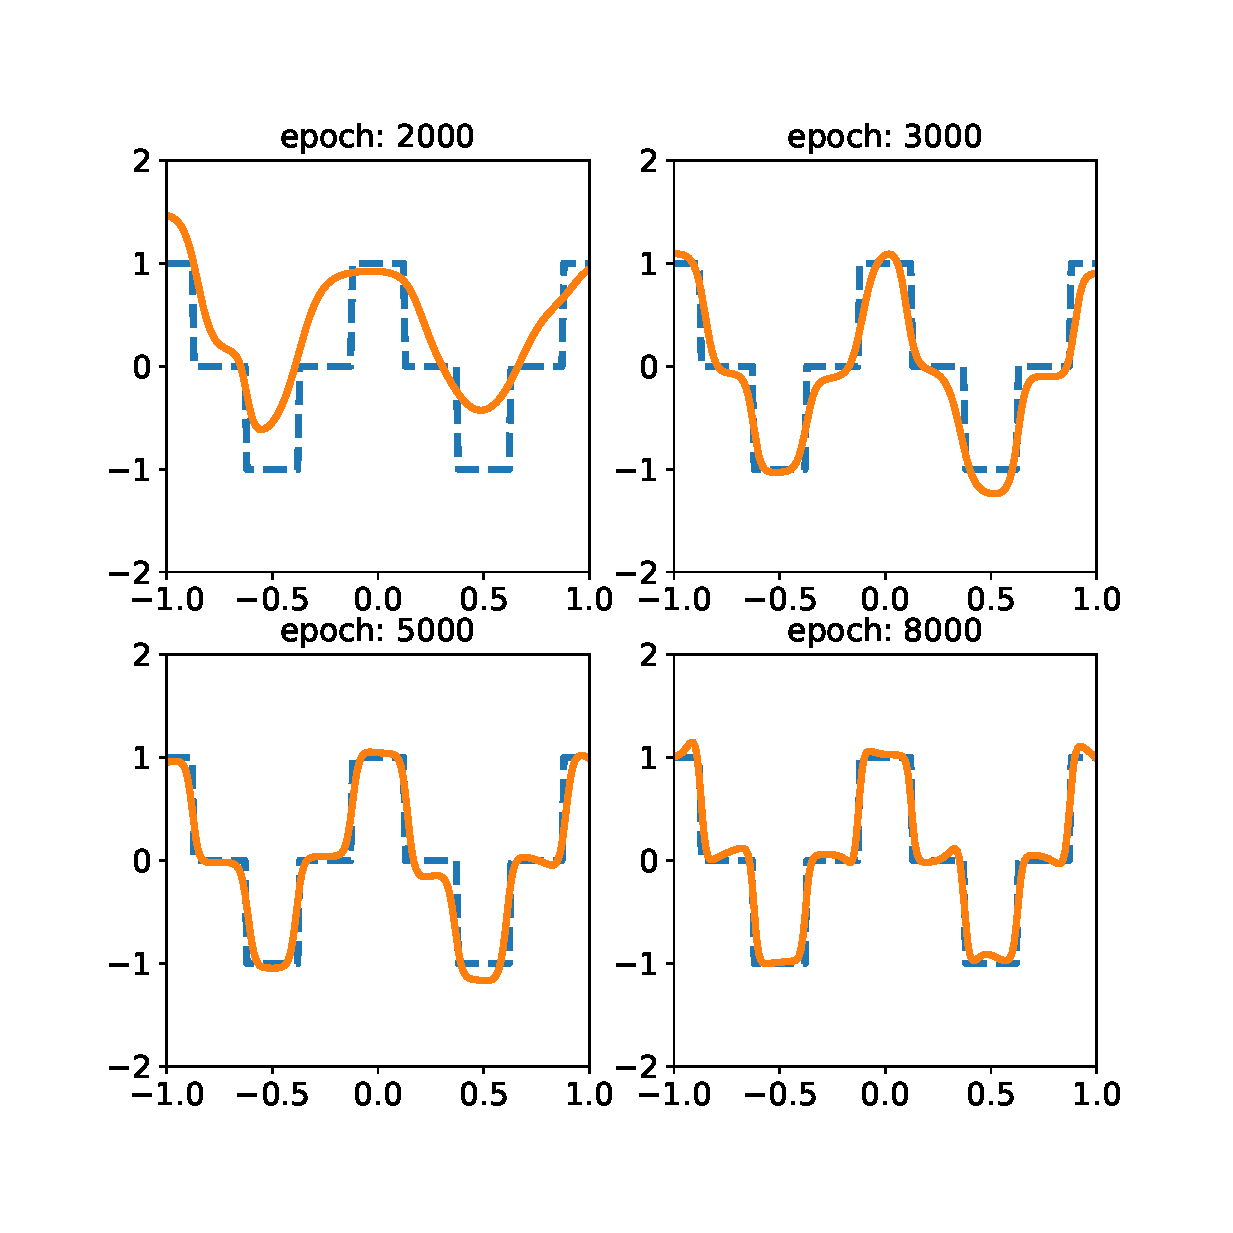
\includegraphics[width=0.6\linewidth]{Figure/Fprinciple_exm2}
	\caption{Approximating function \eqref{equ:target 2} using a network with $n = 50$, $m = 3$, and $2701$ parameters in total. The learning rate is $\lambda=0.2$. $N = 500$ particles and $M=5$ particles for each batch are used in the first $50000$ iterations. After that, the random term is ignored and $M = 10$ is used for faster convergence to the optimal solution.}
	\label{fig:fprincipleexm2}
\end{figure}	
\end{frame}
\begin{frame}
 We use DNNs with a fixed width $10$ and different depths to approximate the function
\begin{equation}\label{func3}
	u(x) = \sin(k\pi x ^k).
\end{equation} 
Set $N = 500$ particles, $M = 5$ particles for each batch.
\begin{table}
	\centering
	\begin{tabular}{|c|c|c|c|c|}
	\hline
		 depth & Num of parameters & k = 2 &  k = 3 & k = 4  \\
		\hline
		4   & 141 & 6.62 e-03 & 1.32 e-02 & 1.71 e-01\\
		7   & 471 & 4.78 e-03 & 1.42 e-02 & 7.54 e-03\\
		12  & 1021 & 7.44 e-03 & 1.30 e-02 & 5.32 e-02\\
		22  & 2121 & 1.00 e-02 & 1.01 e-02 & 1.21 e-01\\
		\hline
	\end{tabular}
	\caption{Dependence of approximation error measured in absolute $L^2$ norm in terms of network depth for \eqref{func3} when $k=2, 3, 4$.}
	\label{tbl:depth vs accuracy}
\end{table}	

 SGD or Adam will failed to converges well (with final error around $0.3$ in absolute $L^2$ norm) when the network depth is $4$ and $10$, respectively.
\end{frame}
\subsection{DNN Solving PDE}
\begin{frame}
\frametitle{DNN Solving PDE}
We adopt the Deep Ritz method (DRM), which is based on the variational formulation associated to the PDE. Consider an elliptic PDE
\begin{equation}\label{eqn:pde}
\left\{
\begin{aligned}
&-\nabla \cdot ( A(x) \nabla u) = - \sum_{i=1}^d\delta(x_i) & x\in \Omega=[-1,1]^d\\
&u(x) = g(x)  & x\in \partial \Omega
\end{aligned}\right.
\end{equation} 
with
\begin{equation}
	A(x)= 
	\left[\begin{matrix}
		(x_1^2)^{\frac{1}{4}} & & \\
		& \ddots & &\\
		& &  (x_d^2)^{\frac{1}{4}}
	\end{matrix}\right].
\end{equation}

\end{frame}
\begin{frame}
The exact solution $u(x)= \sum_{i=1}^d|x_i|^{\frac{1}{2}}$. One can see that the solution is only in $H^{1/2}(\Omega)$ and has singularities when evaluating its derivative at $x_i =0$. The loss function in DRM reads as 
\begin{equation}
\begin{aligned}
	I[u] =& \int_{\Omega}\frac{1}{2}(\nabla u)^T  A(x)  \nabla u(x)\mathrm{d}x + \sum_{i=1}^d\int_{-1}^{1}\delta(x_i)u(x)\mathrm{d}x_i \\ & + \eta \int_{\partial \Omega} (u(x)-g(x))^2 \mathrm{d}x,
	\end{aligned}
\end{equation}	
\end{frame}
\begin{frame}
\begin{table}[H]
	\centering
	\begin{tabular}{|c|c|c|c|c|c|}
		\hline
		d & n & m &  Activation-Optimizer & $L^2$ error & $L^{\infty}$ error\\
		\hline
		\multirow{4}*{2}&\multirow{4}*{20} & \multirow{4}*{2} & ReLu-Adam & 1.23 e-02 & 9.91 e-02\\
		& &  & ReQu-Adam & 2.22 e-02  & 4.21 e-01 \\
		& &  & sigmoid-Adam & 2.19 e-02 & 3.14 e-01\\
		& &  & $|x|^{0.5}$ - Adam-CBO & 3.96 e-03 & 2.09 e-02\\
		\hline
		\multirow{4}*{4}&\multirow{4}*{40} & \multirow{4}*{2} & ReLu-Adam & 6.72 e-03 & 3.70 e-01\\
		& &  & ReQu-Adam & 1.43 e-02 & 1.10 e -00\\
		& &  & sigmoid-Adam & 7.90 e-03 & 7.66 e -02\\
		& &  & $|x|^{0.5}$ -Adam-CBO & 3.13 e-03 & 9.52 e -02\\
		\hline
	\end{tabular}
\caption{Errors measured in $L^2$ and $L^{\infty}$ norms for \eqref{eqn:pde} by Adam and Adam-CBO methods.}\label{tbl:error_singular_PDE}
\end{table}	
\end{frame}

\begin{frame}
	\begin{figure}
	\subfigure[$L^{\infty}$ error]{
		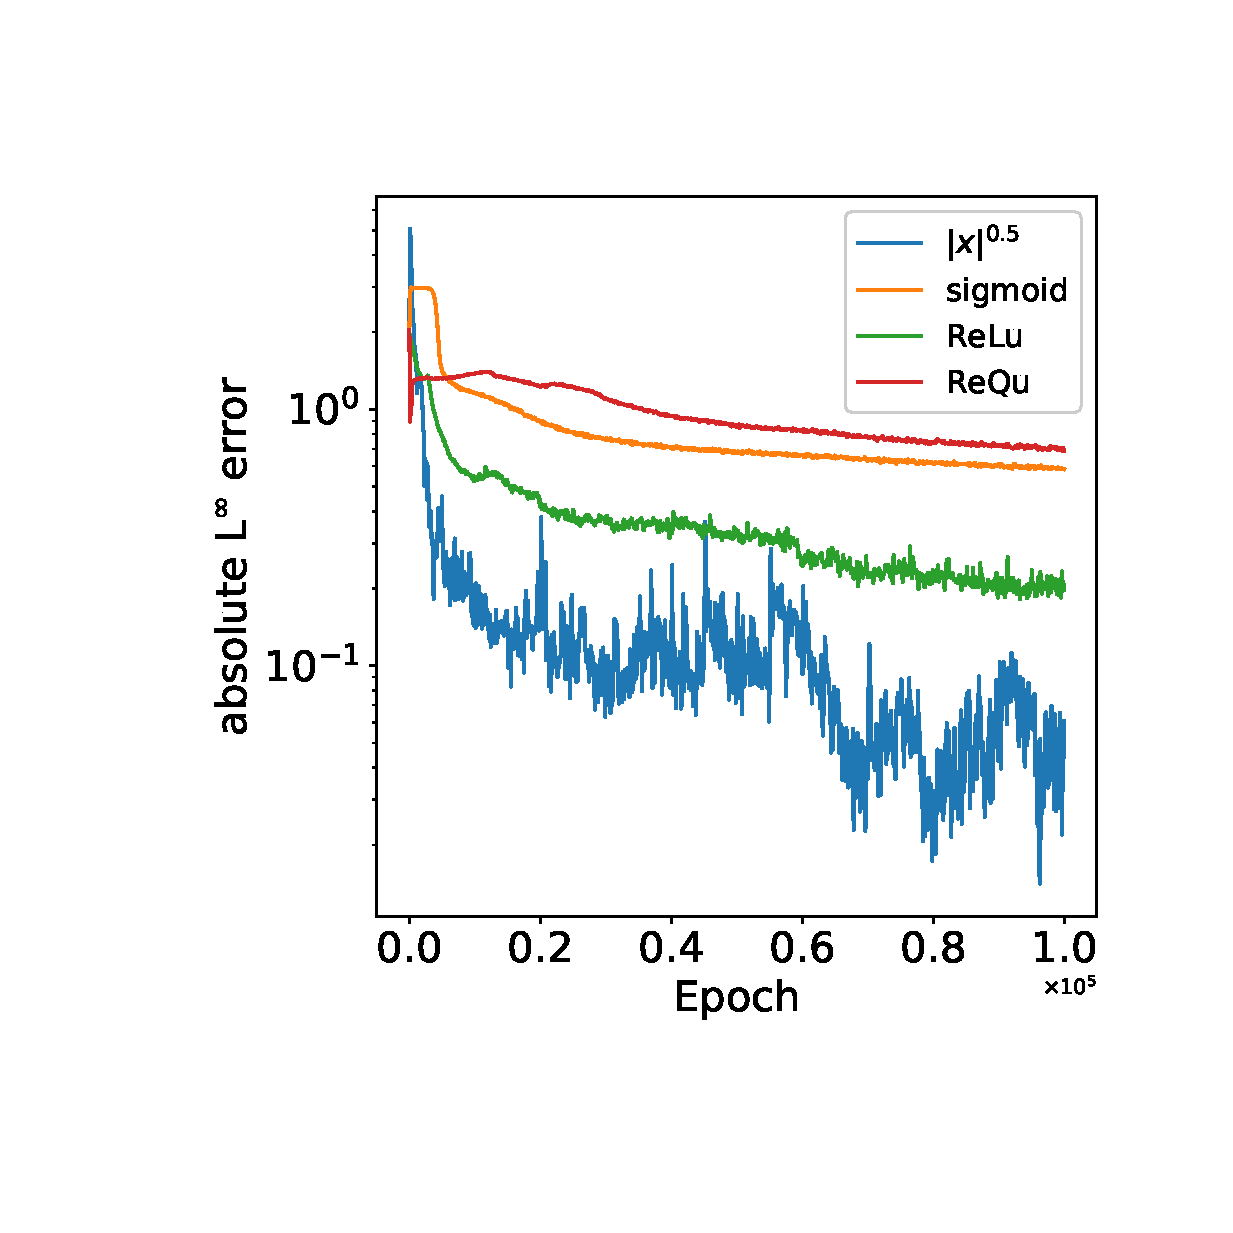
\includegraphics[width=0.45\linewidth]{Figure//singular_PDE_4D_L_infty_error}
	}
	\subfigure[$L^2$ error]{
		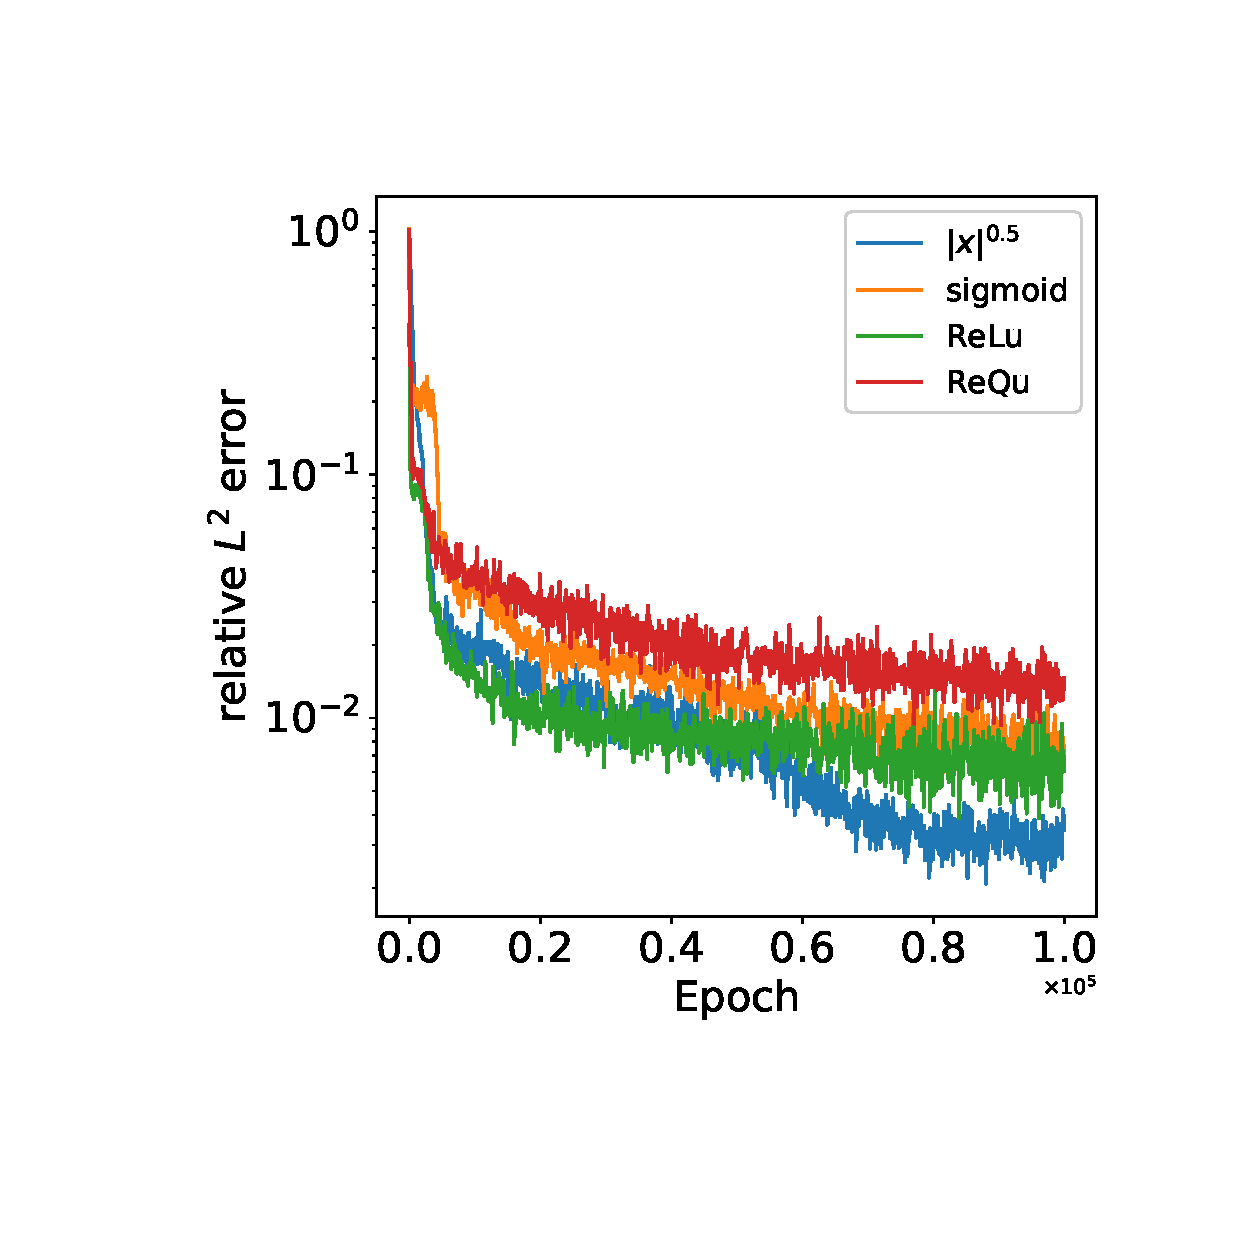
\includegraphics[width=0.45\linewidth]{Figure//singular_PDE_4D_L2_error}
	}
	\caption{Training process of Adam and Adam-CBO methods for \eqref{eqn:pde} when the dimension is $4$. (a) $L^{\infty}$ error; (b) $L^2$ error.}
	\label{fig:training process singular problem}
\end{figure}

\end{frame}
\begin{frame}
\begin{figure}
	\subfigure[$x_2=x_3=x_4=0$]{
		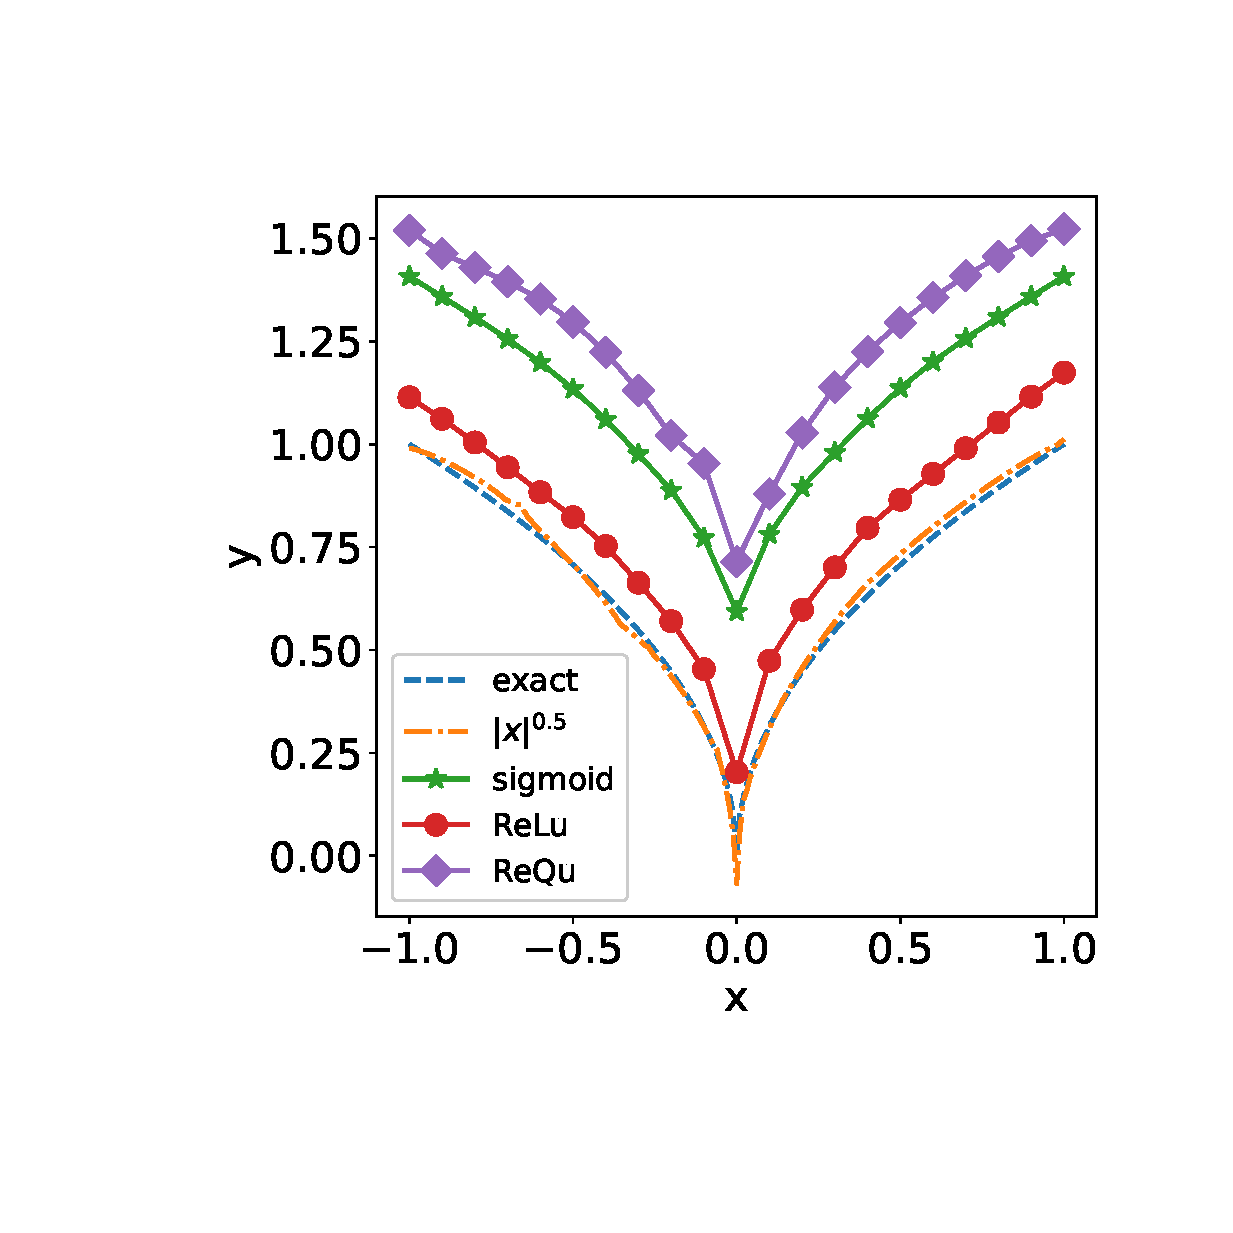
\includegraphics[width=0.45\linewidth]{Figure//singular_PDE_4D_Landscape_x1}
	}
	\subfigure[$x_1=x_3=x_4=0$]{
		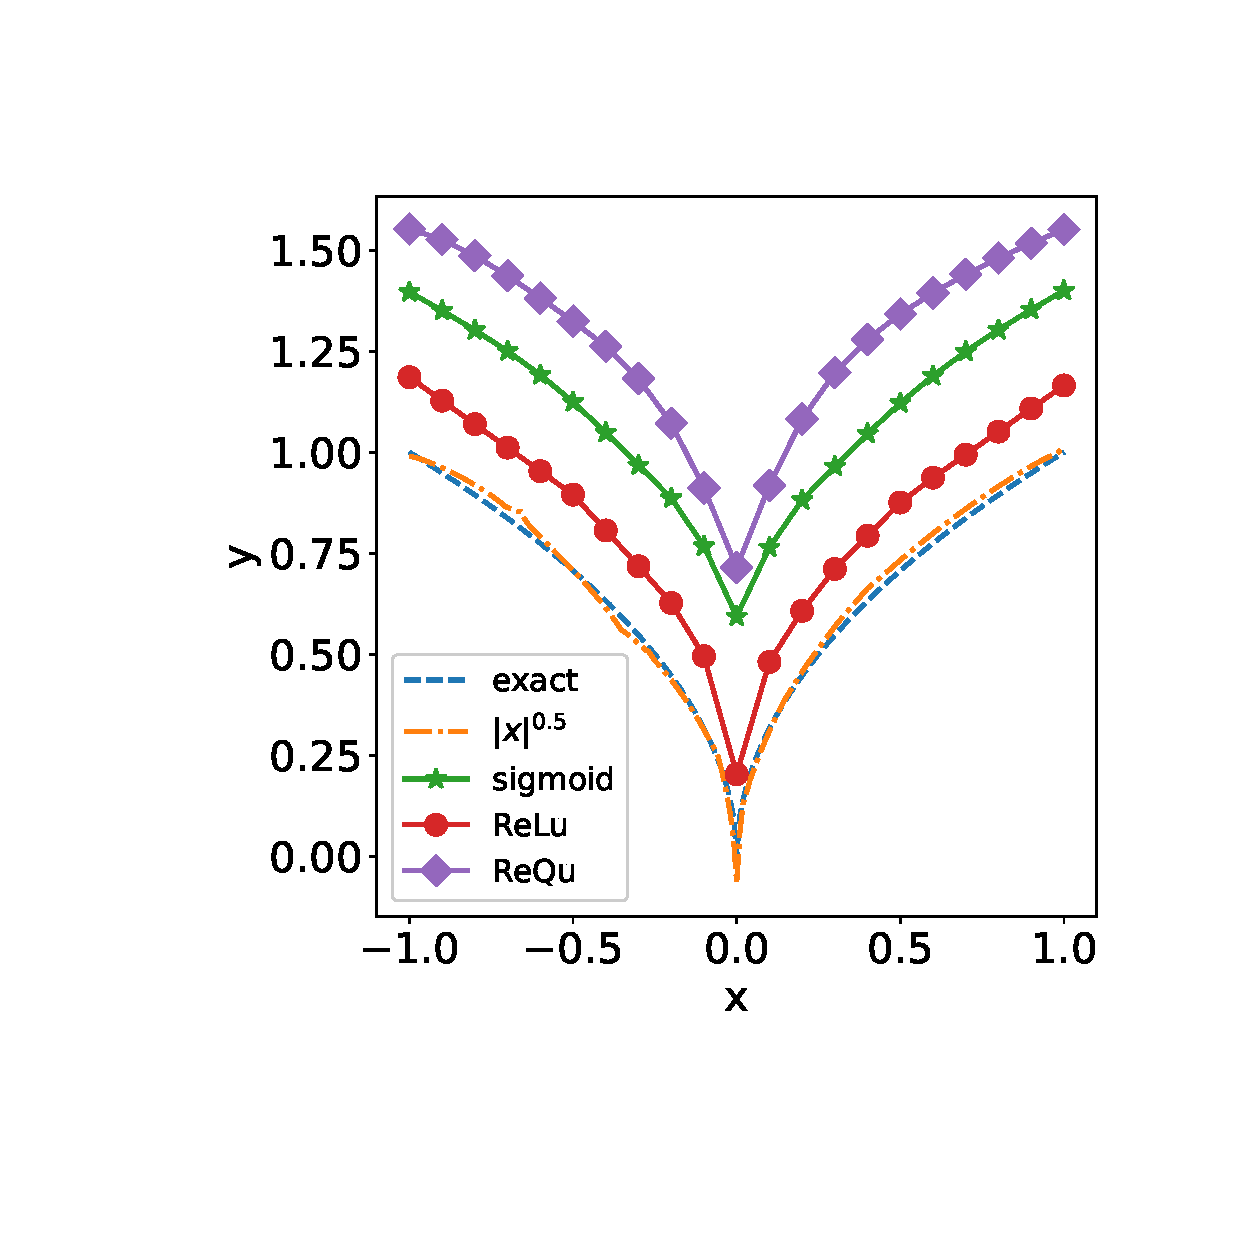
\includegraphics[width=0.45\linewidth]{Figure//singular_PDE_4D_Landscape_x2}
	}
	\caption{One-dimensional solution profiles at the intersection. (a) $x_2=x_3=x_4=0$; (b) $x_1=x_3=x_4=0$;}
\end{figure}	
\end{frame}



\end{document}
